%\fancyfood[R]{\thepage}
%\renewcommand{\headrulewidth}{0.5pt}
\chapter{Design and Practical Implementation}

\chaptermark{Design and Practical Implementation}
\pagestyle{fancy}
\fancyhf{}
\fancyhead[HL]{Chapter 3: Design and Practical Implementation}
\cfoot{\thepage}

\section{Introduction}
The preceding chapters established the project context, defined the platform requirements, 
and presented the hardware components and communication protocols that form the technical 
foundation of the IOBOX platform. This chapter details the design decisions and practical 
implementation work carried out to bring that foundation into a functional embedded system.

The implementation is organized around a layered software architecture that separates 
hardware-specific code from higher-level application logic. At the lowest level, a Board 
Support Package (BSP) provides direct peripheral drivers for every hardware interface 
present on the platform. Above it, a Manager layer encapsulates the communication 
protocols and sensor drivers, exposing clean, hardware-independent APIs to the rest of 
the system. At the top, the Application layer coordinates all modules through a 
lightweight cooperative task scheduler and assembles sensor data into structured 
output frames.

The chapter begins by describing the hardware architecture of the IOBOX platform, 
followed by a detailed account of the software architecture and its constituent layers. 
Each subsection covers the design rationale, the implementation approach, and the key 
technical choices made during development. The chapter concludes with a summary of the 
results obtained and a discussion of the platform's readiness for industrial deployment.
\section{Hardware architecture}


\section{Software Architecture}

The firmware of the IOBOX platform is organised into three distinct horizontal layers: 
the Board Support Package (BSP), the Manager layer, and the Application layer. This 
separation was adopted to isolate hardware-specific code from protocol logic and 
application behaviour, enabling each layer to evolve independently. A central 
configuration file, \texttt{feature\_config.h}, governs the compile-time inclusion of 
every hardware feature through preprocessor flags, ensuring that only the peripherals 
and protocols required for a given deployment are compiled into the firmware binary.

A single global structure, \texttt{SystemBoard}, declared in 
\texttt{feature\_config.h} and instantiated in \texttt{main.c}, serves as the shared 
data exchange point between all layers. It aggregates real-time sensor readings, CAN 
frame data, and status information, and is accessed directly by the Manager and 
Application layers during each execution cycle.

% --- Figure: layered software architecture diagram ---
\begin{figure}[H]
    \centering
    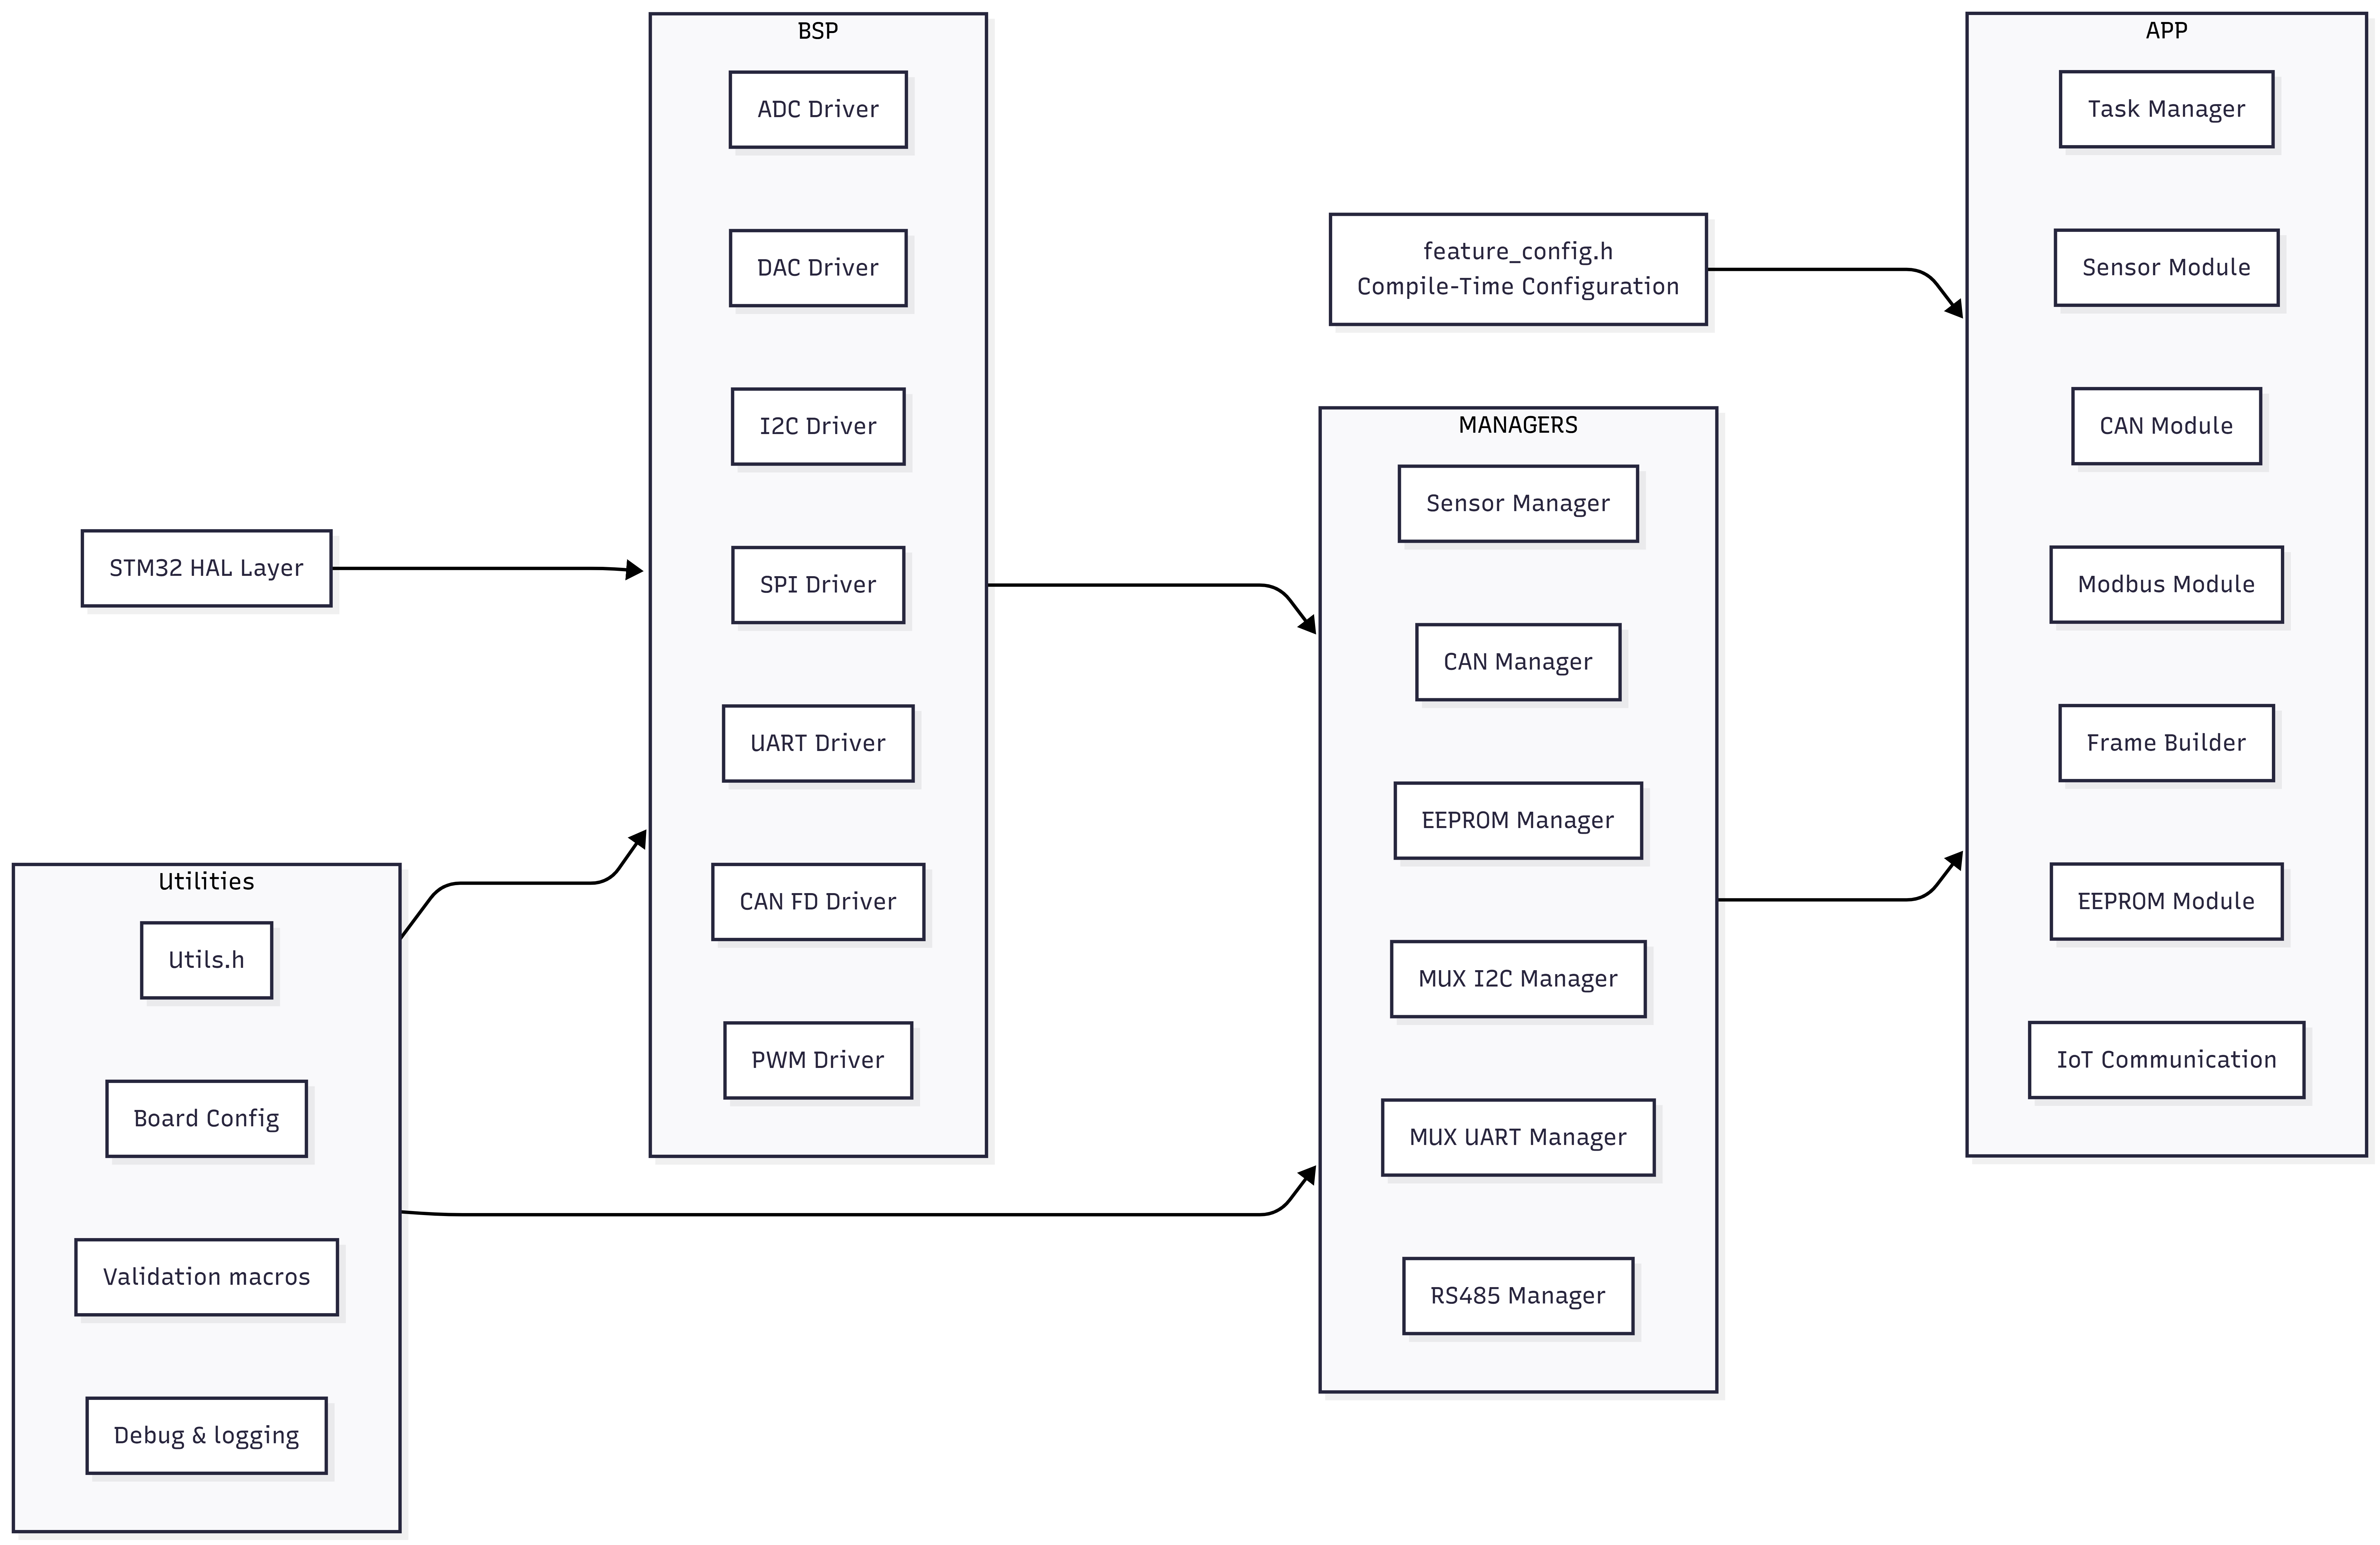
\includegraphics[width=0.75\textwidth]{Figures/software_architecture.png}
    \caption{Layered software architecture of the IOBOX platform}
    \label{fig:software_architecture}
\end{figure}

The following subsections describe each layer in detail, from the lowest hardware 
abstraction level up to the application logic.

%------------------------------------------------------------------
\subsection{Board Support Package Layer}
%------------------------------------------------------------------

The Board Support Package constitutes the lowest layer of the firmware stack. It 
provides a collection of peripheral driver modules, each encapsulating the 
initialisation, configuration, and data transfer routines for a single hardware 
interface. By confining all register-level and HAL-level operations to this layer, the 
upper layers are shielded from hardware-specific details and can interact with 
peripherals exclusively through the BSP's public API.

Each BSP module follows a consistent structure: a header file located under 
\texttt{BSP/Inc/} declares the public API, while the corresponding source file under 
\texttt{BSP/Src/} contains the implementation. The platform exposes BSP modules for the 
following peripheral categories.

Serial communication interfaces are covered by \texttt{BSP\_USART1}, 
\texttt{BSP\_USART2}, \texttt{BSP\_UART5}, and \texttt{BSP\_LPUART1} for general-purpose 
asynchronous communication, by \texttt{BSP\_RS485} for the half-duplex differential bus 
used by the Modbus RTU stack, by \texttt{BSP\_LIN} for the single-wire LIN bus, and by 
\texttt{BSP\_UART\_MUX} for the software-controlled UART channel multiplexer. 
High-speed synchronous communication is handled by three independent SPI drivers: 
\texttt{BSP\_SPI1}, \texttt{BSP\_SPI2}, and \texttt{BSP\_SPI4}. Sensor and 
peripheral expansion buses are served by \texttt{BSP\_I2C2} and \texttt{BSP\_I2C3}, 
complemented by \texttt{BSP\_I2C\_MUX}, which controls the TCA9548A eight-channel I\textsuperscript{2}C 
multiplexer. The CAN interface is abstracted by \texttt{CAN1\_BSP}, and digital 
input/output operations are centralised in \texttt{BSP\_DigitalIO}.

Analog peripherals are equally covered: four ADC drivers (\texttt{ADC1\_BSP}, 
\texttt{ADC3\_BSP}, \texttt{ADC4\_BSP}, \texttt{ADC5\_BSP}) expose acquisition 
functions for each active conversion channel, while two DAC drivers 
(\texttt{BSP\_DAC1} and \texttt{BSP\_DAC2}) provide voltage output generation. 
Four timer drivers (\texttt{TIM1\_BSP} through \texttt{TIM4\_BSP}) manage 
time-base and PWM generation. A low-power management module, \texttt{BSP\_LowPower}, 
groups the power mode transition routines.

This modular decomposition means that porting the firmware to a different STM32 
variant requires changes only within the BSP layer, leaving the Manager and 
Application layers unmodified.

%------------------------------------------------------------------
\subsection{Manager Layer}
%------------------------------------------------------------------
Three sensor manager modules were developed, one per physical sensor, each
handling I\textsuperscript{2}C multiplexer channel selection, register-level communication, and
raw-to-physical conversion.

The HTS221TR manager drives the STMicroelectronics capacitive humidity and
temperature sensor connected to I\textsuperscript{2}C multiplexer channel 0.  Subsequent acquisitions apply linear interpolation between
these reference points to convert the 16-bit raw ADC output into calibrated
temperature in degrees Celsius and relative humidity in percent, as shown in
Equations~\ref{eq:hts_rh} and~\ref{eq:hts_temp}.

\begin{equation}
\label{eq:hts_rh}
\%\mathrm{RH} = H_{0,\mathrm{rH}} +
\frac{(H_{1,\mathrm{rH}} - H_{0,\mathrm{rH}}) \cdot (\mathrm{raw} - H_{0,T_{0}})}
     {H_{1,T_{0}} - H_{0,T_{0}}}
\end{equation}

\begin{equation}
\label{eq:hts_temp}
T\,[^\circ\mathrm{C}] = T_{0,\mathrm{degC}} +
\frac{(T_{1,\mathrm{degC}} - T_{0,\mathrm{degC}}) \cdot (\mathrm{raw} - T_{0,\mathrm{out}})}
     {T_{1,\mathrm{out}} - T_{0,\mathrm{out}}}
\end{equation}

Data readiness is verified by polling the sensor's status register before each
acquisition. If the data-ready flag is not asserted within a configurable retry
count, the acquisition routine returns a timeout status without blocking the
system further.

The ENS210 manager interfaces with the ScioSense combined temperature and
humidity sensor on multiplexer channel~2. The module operates in single-shot
mode: a measurement is triggered by writing to the sensor's start register, a
fixed 10-millisecond settling delay is applied, and the 16-bit raw temperature
and humidity registers are then read. Conversion follows the datasheet-specified
formulae: temperature is obtained as $T_K = \mathrm{raw}/64$, then converted to
Celsius by subtracting 273.15; relative humidity is obtained as
$\%\mathrm{RH} = \mathrm{raw}/512$.

The OPT3001DNPR manager drives the Texas Instruments ambient light sensor on
multiplexer channel~1. The sensor is configured at initialisation by writing a
control word to its configuration register, selecting continuous conversion mode,
automatic full-scale range, and an 800-millisecond conversion time. The 16-bit
result register encodes the measurement as a four-bit binary exponent and a
twelve-bit mantissa; the illuminance in lux is recovered by the expression
$E_{\mathrm{lux}} = \mathrm{mantissa} \times 0.01 \times 2^{\mathrm{exponent}}$.

In all three managers, the I\textsuperscript{2}C multiplexer channel is selected at the start of
each transaction and disabled upon completion, preventing bus contention between
sensors sharing the same physical I\textsuperscript{2}C bus.

\subsubsection{Modbus RTU Manager}

The Modbus RTU stack provides both master and slave roles over the RS485 physical
layer and is entirely self-contained within a single manager module. 
The slave role, which is active in the current platform configuration, operates through
interrupt-driven reception. Eight function codes are supported: FC01, FC02, FC03,
FC04, FC05, FC06, FC15, and FC16. Frames addressed to other slaves are silently
discarded; frames with invalid CRC are dropped without response, as required by the
Modbus RTU specification. Following each handled frame, the receiver is re-armed
immediately to avoid missing subsequent requests.

\subsubsection{CAN Manager}

CAN frame reception is managed by a dedicated module that decouples the 
asynchronous nature of CAN bus traffic from the periodic execution rhythm of 
the Application layer. Because CAN frames can arrive at any time, independently 
of the firmware's scheduling cycle, the manager introduces an intermediate 
buffering stage between the BSP reception interface and the rest of the system. 
Incoming frames are captured and held as they arrive; the Application layer then 
retrieves and consumes them at its own cadence without any risk of frame loss 
during burst traffic conditions. Once processed, the received data is written 
into the CAN-related fields of the shared \texttt{SystemBoard} structure, making 
it immediately available to any other module that consults the platform's central 
data store.
\subsubsection{EEPROM Manager}

Non-volatile data persistence is managed by \texttt{EEPROM\_manager.c}, which 
interfaces with the M95M01-RDW6TP serial EEPROM via the SPI BSP layer. The 
manager exposes store and load primitives consumed by the Application layer to 
persist the \texttt{DataFrame} structure across power cycles.

\subsection{Filter Manager}

Industrial sensor signals are rarely clean: electrical interference, thermal 
gradients, and inherent sensor noise introduce unwanted fluctuations into raw 
measurements that, if left unprocessed, degrade the accuracy of the data 
delivered to the application layer. To address this requirement without coupling 
noise-reduction logic to individual sensor drivers, the IOBOX firmware provides a 
dedicated, generic signal processing module implemented in 
\texttt{Filter\_Manager.c} and \texttt{Filter\_Manager.h}.



The six filter algorithms provided by the module are described individually below.

%------------------------------------------------------------------
\subsubsection{Exponential Moving Average Filter}
%------------------------------------------------------------------

\paragraph{Purpose.}
The Exponential Moving Average (EMA) is a low-pass filter designed to smooth 
noisy sensor readings by weighting recent samples more heavily than older ones 
while discarding neither.

\paragraph{Principle.}
Each output value is a weighted combination of the current raw input and the 
previous filtered output. The weight assigned to the new sample is controlled 
by a single configurable parameter, so the filter can be made to respond quickly 
to real signal changes or to suppress short-lived noise spikes, depending on the 
application.

\paragraph{Main Equation.}
\begin{equation}
    y[n] = \alpha \cdot x[n] + (1 - \alpha) \cdot y[n-1]
    \label{eq:ema}
\end{equation}

\paragraph{Parameters.}
$x[n]$ is the current raw sample, $y[n-1]$ is the previous filtered output 
stored in \texttt{prev\_output}, and $\alpha \in (0,\,1]$ is the smoothing 
factor: values near zero produce heavy smoothing with slow response, while values 
near one allow fast tracking with minimal noise reduction.


\paragraph{Advantages.}
The EMA requires only two floating-point multiplications and one addition per 
update step, making it the least computationally demanding filter in the library. 
Its constant memory footprint and the absence of a ring buffer make it directly 
suitable for resource-constrained microcontrollers. The single parameter 
\texttt{alpha} provides a simple and intuitive tuning knob.

\paragraph{Disadvantages.}
Because all past samples influence the output with exponentially decaying weights, 
the EMA has no finite settling time after a large step change in the input: the 
output approaches the new level asymptotically. Additionally, the degree of 
smoothing depends implicitly on the sampling rate; if the rate changes, the 
effective cutoff behaviour changes as well unless \texttt{alpha} is retuned.

\paragraph{Use within the IOBOX.}
The EMA is the recommended starting filter for continuous sensor channels such 
as the temperature readings from the HTS221TR and ENS210 sensors, where 
measurements arrive at a fixed 1000~ms period and the primary concern is 
reducing high-frequency noise without introducing noticeable lag.

%------------------------------------------------------------------
\subsubsection{Simple Moving Average Filter}
%------------------------------------------------------------------

\paragraph{Purpose.}
The Simple Moving Average (SMA) is a low-pass filter that smooths a signal by 
computing the arithmetic mean of a fixed number of the most recent samples. 
It is used when a consistent, equal-weighted average over a sliding observation 
window is preferred over recursive weighting.

\paragraph{Principle.}
A fixed-size window of recent samples is maintained in a circular ring buffer. 
As each new sample arrives, it replaces the oldest value in the buffer and the 
average is recomputed. A running sum is maintained so that the average requires 
only a subtraction, an addition, and a division per update, rather than 
recomputing the full sum from scratch.

\paragraph{Main Equation.}
\begin{equation}
    y[n] = \frac{1}{N} \sum_{k=0}^{N-1} x[n-k]
    \label{eq:sma}
\end{equation}

\paragraph{Parameters.}
$N$ is the window size, configurable between 1 and \texttt{FILTER\_SMA\_MAX\_WINDOW} 
(defined as 30 in \texttt{Filter\_Manager.h}). $x[n-k]$ represents the sample 
collected $k$ steps before the current one.

\paragraph{Advantages.}
Each sample contributes equally to the output, which gives the SMA a more 
predictable and uniform averaging behaviour than the EMA. The constant-time 
update algorithm means that increasing the window size does not increase 
computational cost per step.

\paragraph{Disadvantages.}
Memory consumption scales linearly with window size: a window of $N$ samples 
requires $N$ floating-point values in the ring buffer, equivalent to $4N$ bytes. 
The maximum window of 30 samples therefore consumes up to 120 bytes per instance. 
The SMA also introduces a latency of $(N-1)/2$ samples before it fully reflects 
a step change in the input.

\paragraph{Use within the IOBOX.}
The SMA is applicable to channels where equal weighting of historical samples is 
required or where the averaging window has a direct physical meaning, such as 
computing a one-minute average of lux readings from the OPT3001DNPR sensor by 
setting $N$ equal to the number of 1000~ms samples in sixty seconds.

%------------------------------------------------------------------
\subsubsection{First-Order IIR High-Pass Filter}
%------------------------------------------------------------------

\paragraph{Purpose.}
The first-order IIR high-pass filter removes slow-varying components and DC 
offsets from a signal, retaining only its dynamic, rapidly changing parts. It 
is used when baseline drift or long-term bias needs to be eliminated from a 
sensor channel.

\paragraph{Principle.}
The filter computes each output as a scaled combination of the current 
input-to-input difference and the previous output. A configurable 
parameter $\alpha$ controls how aggressively the low-frequency content is 
suppressed.

\paragraph{Main Equation.}
\begin{equation}
    y[n] = \alpha \cdot \bigl(y[n-1] + x[n] - x[n-1]\bigr)
    \label{eq:hp_iir}
\end{equation}

\paragraph{Parameters.}
$x[n]$ is the current input, $x[n-1]$ is the previous input stored in 
\texttt{prev\_input}, $y[n-1]$ is the previous output stored in 
\texttt{prev\_output}, and $\alpha \in (0,\,1]$ is the filter coefficient.

\paragraph{Advantages.}
The IIR high-pass filter is computationally inexpensive, requiring three 
additions and one multiplication per update step. Its three-variable state makes 
it one of the most memory-efficient options for baseline removal available in 
the library.

\paragraph{Disadvantages.}
The output depends on both the current and past inputs and outputs, which means 
the filter introduces a phase shift that varies with the rate of change of 
the signal. This can make it less suitable for applications that require 
time-accurate detection of transient events.

\paragraph{Use within the IOBOX.}
This filter is appropriate for removing slow thermal drift from temperature 
sensor readings when only the rate of change or transient excursions are of 
interest to the application, rather than absolute values.

%------------------------------------------------------------------
\subsubsection{Simple Difference High-Pass Filter}
%------------------------------------------------------------------

\paragraph{Purpose.}
The simple difference filter is the most basic high-pass operation available 
in the library. It extracts the sample-to-sample variation of a signal, 
effectively computing a discrete approximation of its rate of change.

\paragraph{Principle.}
Each output value is simply the difference between the current input sample 
and the immediately preceding one. No configurable parameters are involved, 
making this filter parameter-free and ready to use without any tuning.

\paragraph{Main Equation.}
\begin{equation}
    y[n] = x[n] - x[n-1]
    \label{eq:difference}
\end{equation}

\paragraph{Parameters.}
$x[n-1]$ is the previous raw input value, stored in the \texttt{prev\_input} 
field of the \texttt{difference} sub-structure.

\paragraph{Advantages.}
The difference filter imposes the lowest possible computational and memory cost 
of all filters in the library: one subtraction and one assignment per update, 
with one floating-point state variable. It requires no configuration and is 
immediately deployable on any sensor channel.

\paragraph{Disadvantages.}
Because it amplifies high-frequency components of the signal in proportion to 
their frequency, the difference filter is sensitive to high-frequency noise. 
It is appropriate only for channels that are already relatively clean or 
pre-filtered, or for applications where noise spikes and true events can be 
distinguished by magnitude.

\paragraph{Use within the IOBOX.}
The difference filter is suited to event detection on slowly sampled sensor 
channels, such as detecting an abrupt change in ambient light measured by the 
OPT3001DNPR, where a sudden illumination change produces a clearly distinguishable 
output spike against a near-zero background.

%------------------------------------------------------------------
\subsubsection{SMA-Subtraction High-Pass Filter}
%------------------------------------------------------------------

\paragraph{Purpose.}
The SMA-subtraction filter is a high-pass filter that isolates rapid signal 
variations by removing the local moving average from each sample. It provides 
baseline removal with the same ring-buffer mechanism used by the SMA low-pass 
filter, yielding a complementary pair whose outputs sum exactly to the original 
signal.

\paragraph{Principle.}
A sliding window moving average of the input is computed at each step using the 
same efficient running-sum ring-buffer technique as the SMA low-pass filter. The 
high-pass output is then obtained by subtracting this local average from the 
current raw sample.

\paragraph{Main Equation.}
\begin{equation}
    y[n] = x[n] - \frac{1}{N}\sum_{k=0}^{N-1} x[n-k]
    \label{eq:sma_sub}
\end{equation}

\paragraph{Parameters.}
$N$ is the window size, subject to the same constraint as the SMA low-pass: 
clamped to $[1,\,\texttt{FILTER\_SMA\_MAX\_WINDOW}]$.


\paragraph{Advantages.}
Because the high-pass output is derived by subtracting a low-pass output, the 
signal is decomposed without any information loss: the two components always 
reconstruct the original sample exactly. The window size parameter has a direct 
and intuitive interpretation as the time span over which the local baseline is 
estimated.

\paragraph{Disadvantages.}
Memory usage is identical to the SMA low-pass filter: up to 120 bytes per 
instance at the maximum window size. The filter also introduces the same startup 
transient as the SMA: during the first $N-1$ samples, the baseline estimate is 
computed over fewer than $N$ values, which may cause the high-pass output to 
be inaccurate until the buffer is filled.

\paragraph{Use within the IOBOX.}
This filter is well suited to separating short-duration illuminance events from 
slowly evolving ambient light baselines on the OPT3001DNPR channel, or to 
detecting rapid humidity transients against a slowly drifting background on 
either of the two humidity sensor channels.

%------------------------------------------------------------------
\subsubsection{One-State Position Kalman Filter}
%------------------------------------------------------------------

\paragraph{Purpose.}
The one-state Kalman filter provides an optimal estimate of a slowly changing 
scalar quantity by balancing the uncertainty in its own internal model against 
the uncertainty in each new measurement. It adapts its smoothing behaviour 
automatically over time, without requiring manual tuning of a fixed coefficient.

\paragraph{Principle.}
At each step, the filter first predicts how much its confidence in the current 
estimate has degraded (the prediction step), then corrects the estimate using 
the new measurement weighted by a dynamically computed gain (the update step). 
The gain is large when the filter is uncertain and small when it is confident, 
allowing it to track real changes quickly at startup and to suppress noise 
efficiently at steady state.

\paragraph{Main Equations.}
\begin{align}
    K &= \frac{P + Q}{P + Q + R} \label{eq:kalman1_gain} \\[4pt]
    \hat{x} &= \hat{x} + K \cdot (z - \hat{x}) \label{eq:kalman1_state} \\[4pt]
    P &= (1 - K)\,(P + Q) \label{eq:kalman1_cov}
\end{align}

\paragraph{Parameters.}
$Q$ is the process noise variance (\texttt{process\_variance}), reflecting how 
much the true quantity is expected to vary between samples; $R$ is the 
measurement noise variance (\texttt{measurement\_variance}), reflecting sensor 
noise power; $\hat{x}$ is the current state estimate (\texttt{state\_estimate}); 
$P$ is the estimation error covariance (\texttt{error\_covariance}); $z$ is the 
new measurement; and $K$ is the Kalman gain computed at each step.


\paragraph{Advantages.}
The one-state Kalman filter adapts its smoothing level automatically: it applies 
less smoothing early in a measurement session (when uncertainty is high) and 
progressively more as confidence accumulates. This eliminates the need to choose 
a fixed smoothing coefficient and makes the filter more robust to varying signal 
conditions than either the EMA or SMA. Its memory footprint is fixed at four 
floating-point variables regardless of operating conditions.

\paragraph{Disadvantages.}
The filter assumes that the true quantity changes only due to random, 
zero-mean process noise (constant-position model). If the quantity exhibits a 
systematic trend — such as a steadily rising temperature — the filter will lag 
behind the true value, because the model does not account for a rate of change. 
The two-state velocity filter described below addresses this limitation.

\paragraph{Use within the IOBOX.}
The position Kalman filter is the most suitable algorithm for the temperature 
and humidity channels of the HTS221TR and ENS210 sensors under stable operating 
conditions, where the physical environment changes slowly and randomly. It is 
particularly appropriate in deployments where sensor noise characteristics 
are known and $Q$ and $R$ can be set from datasheet specifications or 
empirical characterisation.

%------------------------------------------------------------------
\subsubsection{Two-State Constant-Velocity Kalman Filter}
%------------------------------------------------------------------

\paragraph{Purpose.}
The two-state Kalman filter extends the position model by additionally tracking 
the rate of change (velocity) of the measured quantity. It is designed for 
signals that exhibit persistent trends rather than stationary fluctuations around 
a fixed value.

\paragraph{Principle.}
The filter maintains a two-element state vector containing position and velocity. 
At each step, the prediction phase advances the position estimate by the current 
velocity estimate, then corrects both using the new measurement. The correction 
is distributed between position and velocity through two separate gain values, 
computed from a 2×2 covariance matrix that tracks the uncertainty in each state.

\paragraph{Main Equation.}
The state prediction is:
\begin{equation}
    \begin{bmatrix} \hat{x}_{\text{pos}} \\ \hat{x}_{\text{vel}} \end{bmatrix}_{n}^{-}
    =
    \begin{bmatrix} 1 & 1 \\ 0 & 1 \end{bmatrix}
    \begin{bmatrix} \hat{x}_{\text{pos}} \\ \hat{x}_{\text{vel}} \end{bmatrix}_{n-1}
    \label{eq:kalman2_predict}
\end{equation}
followed by a measurement-driven correction of both state components using 
gains $K_{\text{pos}}$ and $K_{\text{vel}}$ computed from the updated 
2×2 covariance matrix.

\paragraph{Parameters.}
The filter is configured with a diagonal 2×2 process noise matrix $\mathbf{Q}$ 
(fields \texttt{process\_noise[0]} for position noise and \texttt{process\_noise[3]} 
for velocity noise), a scalar measurement noise variance $R$ 
(\texttt{measurement\_noise}), an initial state vector 
\texttt{state[2]~=~[init\_pos, init\_vel]}, and a diagonal initial covariance 
matrix with \texttt{init\_cov\_pos} and \texttt{init\_cov\_vel} on the diagonal. 
Off-diagonal covariance terms are initialised to \texttt{0.0f}.


\paragraph{Advantages.}
By explicitly tracking velocity, this filter anticipates trends in the signal 
and tracks them with lower latency than the position-only model under equivalent 
noise conditions. It is the most general-purpose filter in the library for 
non-stationary signals.

\paragraph{Disadvantages.}
The two-state filter is the most computationally intensive in the library, 
requiring the full expand of a 2×2 matrix predict–update cycle at each step. 
It also requires more parameters to tune: both process noise terms and the 
initial velocity estimate must be chosen appropriately. Memory usage amounts to 
ten floating-point variables per instance (\texttt{state[2]}, 
\texttt{covariance[4]}, \texttt{process\_noise[4]}, and 
\texttt{measurement\_noise}).

\paragraph{Use within the IOBOX.}
This filter is appropriate for sensor channels that are expected to exhibit 
systematic trends during normal operation, such as temperature measurements 
taken during equipment warm-up or cool-down cycles, where the temperature rises 
or falls at a measurable rate that the position-only model would fail to track 
accurately.

%------------------------------------------------------------------
\subsubsection{Filter Manager: Architectural Summary}
%------------------------------------------------------------------

The Filter Manager provides the IOBOX firmware with a complete, self-contained 
signal processing toolkit whose design is driven by three embedded-systems 
constraints: zero dynamic memory allocation, constant-time dispatch, and a 
uniform calling interface. Table~\ref{tab:filter_summary} summarises the 
computational and memory characteristics of each filter.

\begin{table}[H]
    \centering
    \caption{Computational and memory characteristics of the Filter Manager algorithms}
    \label{tab:filter_summary}
    \begin{tabular}{|l|l|c|c|}
        \hline
        \textbf{Category} & \textbf{Method} & \textbf{State Variables} & \textbf{Ops per Update} \\
        \hline
        Low-pass  & EMA                  & 2          & 3 \\
        \hline
        Low-pass  & SMA                  & $N + 3$    & 4 \\
        \hline
        High-pass & IIR                  & 3          & 4 \\
        \hline
        High-pass & Difference           & 1          & 1 \\
        \hline
        High-pass & SMA-Subtraction      & $N + 3$    & 5 \\
        \hline
        Kalman    & Position (1-state)   & 4          & 6 \\
        \hline
        Kalman    & Velocity (2-state)   & 10         & $\approx$20 \\
        \hline
    \end{tabular}
\end{table}

Any sensor channel in the firmware can be filtered by declaring a 
\texttt{FilterInstance\_t} variable, calling the appropriate initialisation 
function once, and then passing each new raw measurement to 
\texttt{Filter\_Update()} to obtain the processed value. The choice of algorithm 
depends on the signal characteristics and the computational budget available: 
the EMA and difference filters are the lightest options for high-rate channels, 
while the Kalman filters offer adaptive, statistically grounded noise reduction 
for channels where noise parameters can be characterised.
%------------------------------------------------------------------
\subsection{Application Layer}
%------------------------------------------------------------------

The Application layer is the topmost layer of the firmware stack. It does not 
interact with hardware directly but instead coordinates the Manager modules, 
orchestrates data flow, and assembles the final output frame. It is composed of 
four modules: the cooperative task scheduler, the Sensor Module, the Modbus 
Module, and the Frame Builder.

\subsubsection{Cooperative Task Scheduler}

Rather than employing a real-time operating system, a lightweight cooperative 
scheduler was implemented directly in \texttt{main.c}. The scheduler is based on 
a statically allocated array of \texttt{TaskEntry} structures, each holding a 
function pointer (\texttt{task\_fn}), a period in milliseconds 
(\texttt{period\_ms}), and a timestamp of the last execution 
(\texttt{last\_ms}). The dispatcher \texttt{Application\_RunTasks()} iterates 
over the array on every pass of the main loop and invokes each task function 
whenever the elapsed time since its last execution meets or exceeds its 
configured period.

Six tasks are registered in the current configuration, as shown in 
Table~\ref{tab:task_schedule}. All task functions are non-blocking by design: 
they return immediately if no new data is available or if their internal period 
has not elapsed, preventing any single task from starving the others.

\begin{table}[H]
    \centering
    \caption{Registered tasks in the cooperative scheduler}
    \label{tab:task_schedule}
    \begin{tabular}{|l|c|l|}
        \hline
        \textbf{Task Function} & \textbf{Period (ms)} & \textbf{Responsibility} \\
        \hline
        \texttt{SensorModule\_Task}  & 10   & Poll all enabled sensors \\
        \hline
        \texttt{CAN\_Manager\_Run}   & 10   & Drain CAN FIFO and update \texttt{sysboard.can} \\
        \hline
        \texttt{Modbus\_Module\_Poll} & 20  & Process incoming Modbus RTU frames \\
        \hline
        \texttt{EEPROM\_StoreFrame}  & 1000 & Persist current \texttt{SystemBoard} to EEPROM \\
        \hline
        \texttt{EEPROM\_LoadTask}    & 1000 & Reload last stored frame from EEPROM \\
        \hline
        \texttt{FrameBuilderTask}    & 1000 & Assemble and finalise the output \texttt{IoFrame} \\
        \hline
    \end{tabular}
\end{table}

\subsubsection{Sensor Module}

The Sensor Module, implemented in \texttt{Sensor\_module.c}, provides a unified 
acquisition interface for all enabled sensors. It maintains one private 
timestamp variable per sensor and, on each invocation of 
\texttt{SensorModule\_Task()}, compares the current tick against each timestamp 
to determine whether the sensor's configured sampling period has elapsed. When it 
has, the corresponding manager acquisition function is called and the result is 
written directly into the \texttt{sysboard} global structure. The per-sensor 
sampling periods are defined centrally in \texttt{feature\_config.h}: 1000~ms 
for the HTS221TR, 1000~ms for the ENS210, and 1000~ms for the OPT3001DNPR. 
The module is fully driven by compile-time feature flags; sensors disabled at 
configuration time introduce no runtime overhead.

\subsubsection{Modbus Application Module}

The Modbus Application Module forms the bridge between the Modbus RTU stack and 
the platform data model. It defines a static register map that associates each 
Modbus register address and object type with the corresponding field in the shared 
\texttt{SystemBoard} structure and an access permission flag. The current 
register map exposes five read-only input registers: ENS210 humidity at 
address~0, ENS210 temperature at address~1, HTS221TR humidity at address~2, 
HTS221TR temperature at address~3, and OPT3001 illuminance at address~4. 
Floating-point values are scaled by a factor of 100 before transmission, 
preserving two decimal places within the 16-bit Modbus register format.

Handlers for each supported function code are registered in the Modbus slave 
handle and invoked by the Modbus Manager dispatcher upon receipt of a valid 
request.

\begin{table}[H]
    \centering
    \caption{Modbus input register map}
    \label{tab:modbus_map}
    \begin{tabular}{|c|l|l|c|}
        \hline
        \textbf{Address} & \textbf{Source} & \textbf{Physical Quantity} & \textbf{Scale} \\
        \hline
        0 & ENS210 humidity field   & Relative humidity (\%) & $\times 100$ \\
        \hline
        1 & ENS210 temperature field & Temperature (°C)      & $\times 100$ \\
        \hline
        2 & HTS221TR humidity field  & Relative humidity (\%) & $\times 100$ \\
        \hline
        3 & HTS221TR temperature field & Temperature (°C)    & $\times 100$ \\
        \hline
        4 & OPT3001 illuminance field & Illuminance (lux)    & $\times 100$ \\
        \hline
    \end{tabular}
\end{table}

\subsubsection{Frame Builder}

The Frame Builder is responsible for assembling the final output structure that 
the IOBOX platform transmits to external systems. Rather than forwarding raw 
sensor readings directly, the platform encapsulates all acquired data within a 
structured binary frame whose layout is illustrated in 
Figure~\ref{fig:ioframe_structure}. This design ensures that any receiving system 
can unambiguously identify, validate, and decode the payload regardless of which 
sensors or modules are active in a given deployment.

\begin{figure}[H]
    \centering
    
\includegraphics[width=\textwidth]{Figures/ioframe_structure.png}
    \caption{Structure of the IOBOX output frame}
    \label{fig:ioframe_structure}
\end{figure}

The frame assembly routine populates each field from the most recently 
persisted system state, then computes and appends a CRC checksum over all 
preceding fields. The complete frame format is described in detail below.

\paragraph{Start Byte.}
A fixed synchronisation marker (\texttt{0xAA}) that signals the beginning of a 
valid frame to any receiver scanning an incoming byte stream, allowing frame 
boundaries to be established without relying on inter-frame timing gaps.

\paragraph{Device Type.}
Identifies the category of the transmitting device, allowing a network to host 
multiple types of embedded nodes simultaneously. A receiving gateway inspects 
this field to apply the appropriate decoding logic without prior knowledge of 
the sender's identity.

\paragraph{IOBOX ID.}
Carries the unique numeric identifier of the specific IOBOX unit that generated 
the frame. In multi-node deployments, this field allows a receiving system to 
associate each frame with its physical origin without requiring any session or 
connection establishment.

\paragraph{Mask ID.}
A configuration bitmap describing which sensors and communication modules are 
active and contributing data to the current frame. Each bit corresponds to one 
module, as detailed in Table~\ref{tab:mask_id}. The receiver reads this field 
before parsing the payload to determine the exact byte layout of the Data field, 
providing both flexibility and forward compatibility.

\begin{table}[H]
    \centering
    \caption{Mask ID bit field definitions}
    \label{tab:mask_id}
    \begin{tabular}{|c|l|c|}
        \hline
        \textbf{Bit} & \textbf{Module} & \textbf{Logic 1 meaning} \\
        \hline
        5 & CAN sniffer             & CAN data present in payload \\
        \hline
        4 & HTS221TR Temperature    & HTS221 temperature present \\
        \hline
        3 & HTS221TR Humidity       & HTS221 humidity present \\
        \hline
        2 & ENS210 Temperature      & ENS210 temperature present \\
        \hline
        1 & ENS210 Humidity         & ENS210 humidity present \\
        \hline
        0 & OPT3001DNPR Illuminance & OPT3001 lux value present \\
        \hline
    \end{tabular}
\end{table}

\paragraph{Length.}
Specifies the total size of the Data field in bytes, making the frame 
self-describing. The receiver uses this field to locate the CRC and End Byte at 
their correct positions without re-deriving the payload size from the Mask ID.

\paragraph{Data.}
Contains the measurement values and communication data collected during the 
current acquisition cycle. Its contents are governed entirely by the active bits 
in the Mask ID field. In the current configuration, the payload includes 
temperature and humidity readings from both sensor units, the OPT3001DNPR 
illuminance value, and the CAN frame payload comprising the message identifier, 
RTR flag, data length code, and up to eight data bytes.

\paragraph{CRC.}
A 16-bit integrity checksum computed over all preceding fields using the 
CRC-16/IBM polynomial. The receiver verifies this field before consuming any 
measurement data; a mismatch indicates a transmission error or a corrupted frame 
and requires the frame to be discarded.

\paragraph{End Byte.}
A fixed termination marker (\texttt{0x55}) that constitutes a second layer of 
frame boundary validation. Together with the Start Byte, it allows the receiver 
to detect framing errors — for example, those caused by a corrupted Length field 
— even when the CRC alone might not reveal the misalignment.

The complete field layout is summarised in Table~\ref{tab:ioframe_fields}.

\begin{table}[H]
    \centering
    \caption{IoFrame field summary}
    \label{tab:ioframe_fields}
    \begin{tabular}{|l|l|p{6.5cm}|}
        \hline
        \textbf{Field} & \textbf{Value} & \textbf{Description} \\
        \hline
        Start Byte  & \texttt{0xAA}    & Frame synchronisation delimiter \\
        \hline
        Device Type & Compile-time constant & Node category identifier \\
        \hline
        IOBOX ID    & Compile-time constant & Per-unit unique identifier \\
        \hline
        Mask ID     & 6-bit bitmap     & Active module bitmap \\
        \hline
        Length      & Variable         & Data field length in bytes \\
        \hline
        Data        & Variable         & Active measurement payload \\
        \hline
        CRC         & CRC-16/IBM       & Integrity check over all preceding fields \\
        \hline
        End Byte    & \texttt{0x55}    & Frame termination delimiter \\
        \hline
    \end{tabular}
\end{table}

The frame assembly routine retrieves the last persisted system state and fills 
every field sequentially before computing and inserting the CRC. This design 
ensures that the output frame always reflects the most recently stored platform 
state, providing continuity across power cycles and making the frame contents 
auditable through the non-volatile storage layer.
\subsubsection{System Data Flow}

% --- Figure: data flow diagram ---
\begin{figure}[H]
    \centering
    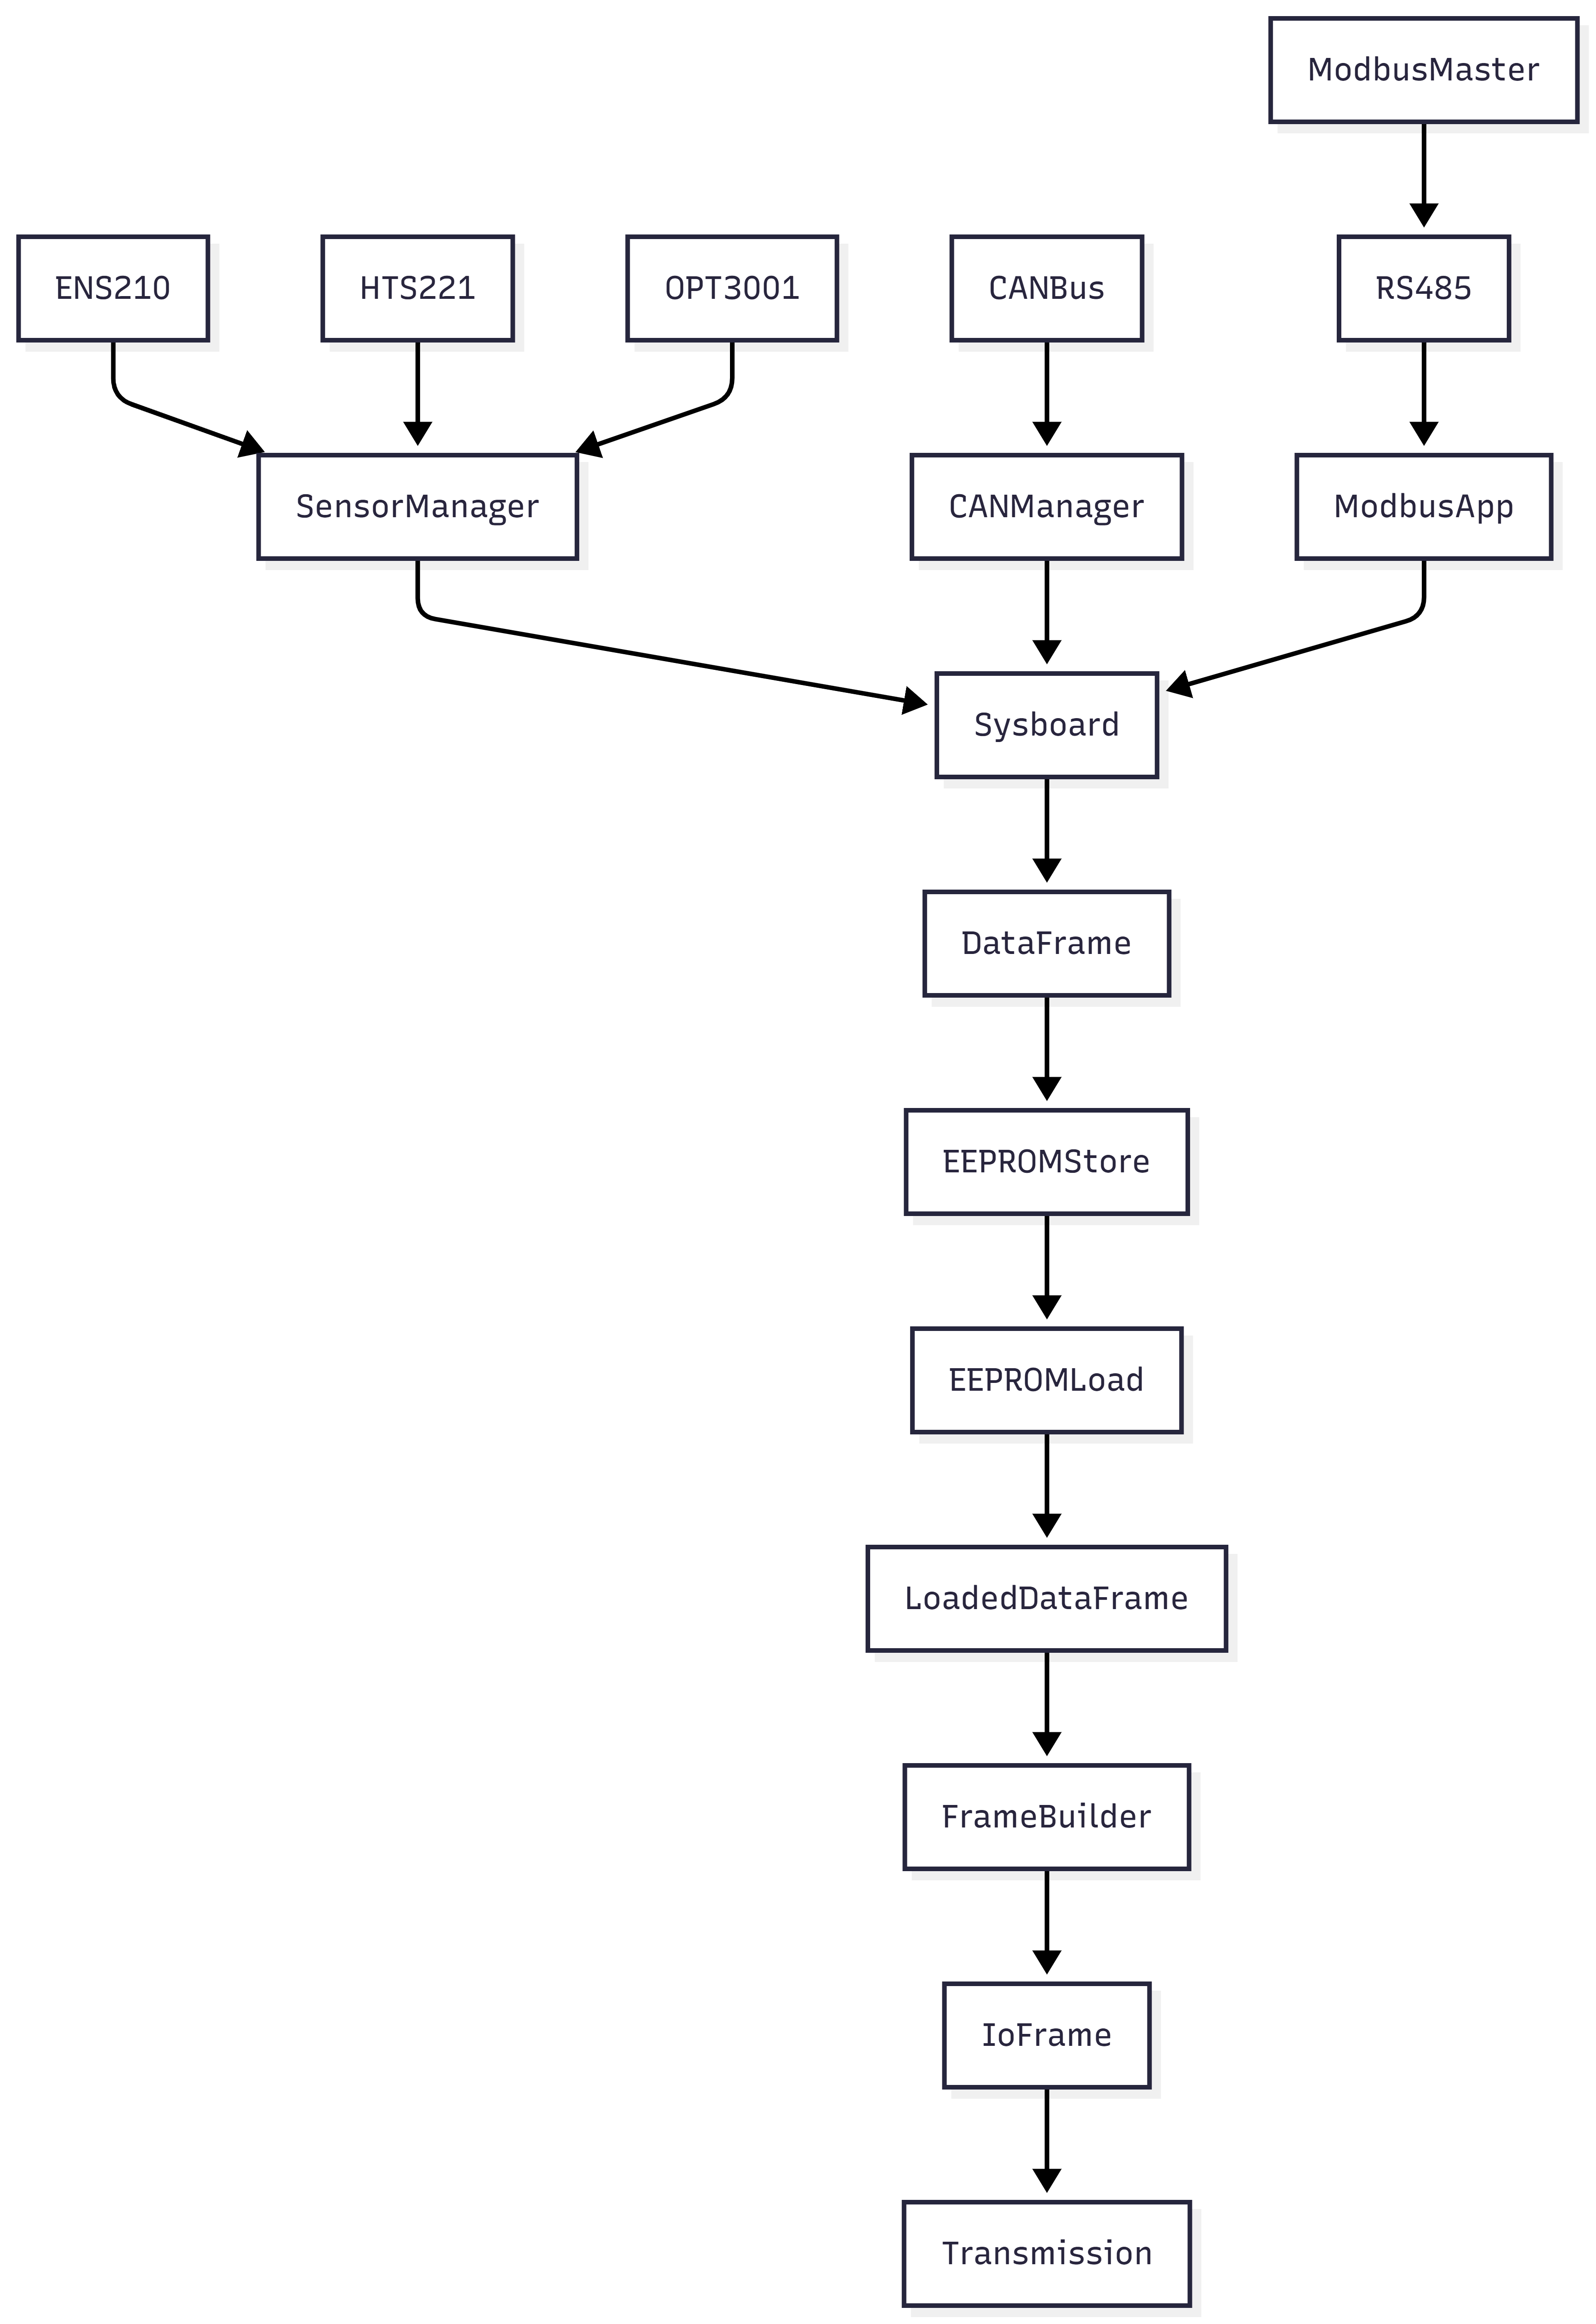
\includegraphics[width=0.85\textwidth]{Figures/data_flow.png}
    \caption{End-to-end data flow across the three firmware layers}
    \label{fig:data_flow}
\end{figure}

The complete data path through the system can be summarised as follows. Physical 
sensor measurements are acquired by the Sensor Module and written into 
\texttt{sysboard}. Simultaneously, CAN frames captured by the CAN Manager are 
stored in the same structure. At every 1000~ms interval, the EEPROM Store task 
serialises \texttt{sysboard} into a \texttt{DataFrame} and writes it to 
non-volatile memory; the EEPROM Load task immediately retrieves the last valid 
frame. Finally, the Frame Builder consumes the loaded \texttt{DataFrame} and 
produces the \texttt{IoFrame} output, ready for transmission. Throughout this 
pipeline, any Modbus master connected via RS485 may read live sensor values 
directly from \texttt{sysboard} through the Modbus Application Module at any 
point in the cycle.

\section*{} % transition placeholder — Conclusion follows
The software architecture described in this section provides a clean separation 
of concerns, compile-time configurability, and a deterministic execution model 
without the overhead of a real-time operating system. The following section 
presents the validation results obtained on the target hardware.

\section{Conclusion}